\documentclass[10pt]{article}
\usepackage[utf8]{inputenc}
\usepackage[T1]{fontenc}
\usepackage{amsmath}
\usepackage{amsfonts}
\usepackage{amssymb}
\usepackage[version=4]{mhchem}
\usepackage{stmaryrd}
\usepackage{graphicx}
\usepackage[export]{adjustbox}
\graphicspath{ {./images/} }

\begin{document}

    A telescope with an achromatic convex objective lens of diameter $D=15 \mathrm{~cm}$ and focal length $f=200 \mathrm{~cm}$ is pointed to a star at the zenith.\\
    (T09.1) Find the diameter (in m ), $d_{\text {image }}$, of the image of a point source as produced by the objective lens at its focal plane for green light ( $\lambda=550 \mathrm{~nm}$ ), considering only the effects of diffraction.
    
    The image of an astronomical source is also affected by the so-called "atmospheric seeing".\\
    The boundaries between the layers in the atmosphere as well as the refractive indices of the layers change continuously due to turbulence, temperature variation and other factors. This leads to tiny changes in the position of the image in the focal plane of the telescope, known as the "twinkling effect". For rest of the problem, apart from using the diffraction limited finite size of the image of the star (as used above), no interference effects will be considered.
    
    The left panel of the figure below shows a vertical cross-section of the atmosphere with multiple layers of different refractive indices ( $n_{1}, n_{2}, n_{3}, \ldots$ ). The right panel shows the zoomed in view of a thin vertical segment of the atmosphere and the boundary between the two lowest atmospheric layers of refractive indices $n_{1}$ and $n_{2}\left(n_{1}>n_{2}\right.$ ). We consider only these two layers and their boundary for this problem. The diagrams are not to scale.\\
    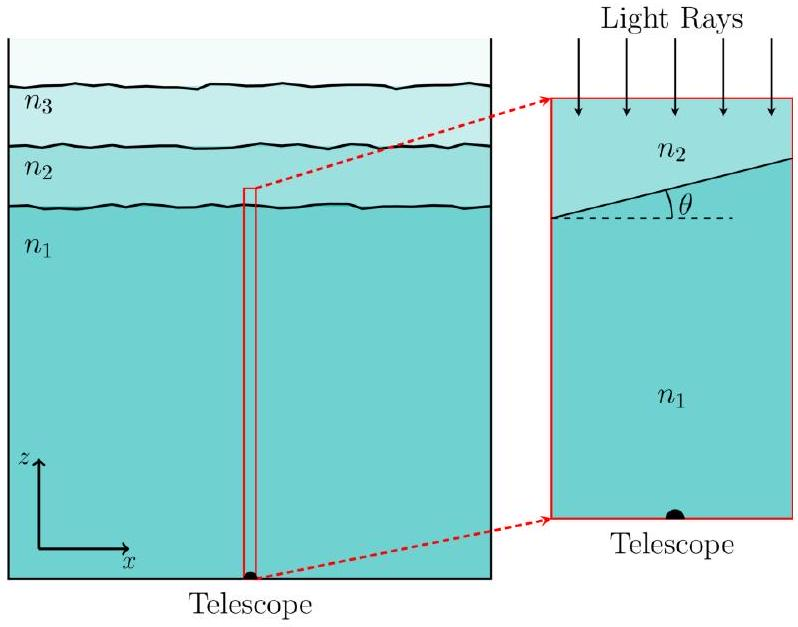
\includegraphics[max width=\textwidth, center]{2025_08_23_e94579452776a99c4850g-09(1)}\\
    (T09.2) Let the boundary between the two layers be at a height $H=1 \mathrm{~km}$ directly above the telescope objective, with a tilt of $\theta=30^{\circ}$ with respect to the horizontal plane. In all parts of this problem $\theta$ is taken to be positive in the anti-clockwise direction. For a monochromatic light source, $n_{1}=1.00027$ and $n_{2}=1.00026$. Let the angular shift of the image at the focal plane of the telescope for a star at the zenith be $\alpha$.\\
    (T09.2a) Draw an appropriately labelled ray-diagram at the boundary showing $n_{1}, n_{2}, \theta$ and $\alpha$.\\
    (T09.2b) Find the expression for $\alpha$ in terms of $\theta, n_{1}$ and $n_{2}$. Use the small angle approximations: $\sin \alpha \approx \alpha$ and $\cos \alpha \approx 1$.\\
    (T09.2c) Calculate the displacement, $\Delta x_{\theta}$ (in m ), in the position of the image if $\theta$ increases by $1 \%$ (keeping $n_{1}$ and $n_{2}$ fixed).\\
    (T09.2d) Calculate the displacement, $\Delta x_{n}$ (in m ), in the position of the image if $n_{2}$ increases by $0.0001 \%$ (keeping $n_{1}$ and $\theta$ fixed).\\
    (T09.3) For white light coming from a star at the zenith, choose which of the following most closely describes the shape and colour of the image by ticking $(\checkmark)$ the appropriate box (only one) in the Summary Answersheet. Note $x$ increases from left to right in the figure.
    
    \begin{center}
    \begin{tabular}{|l|l|l|l|l|}
    \hline
     & Image colour & Image shape & Left edge & Right edge \\
    \hline
    A & White & Circular &  &  \\
    \hline
    B & White & Elliptical &  &  \\
    \hline
    C & Coloured & Circular & Blue & Red \\
    \hline
    D & Coloured & Circular & Red & Blue \\
    \hline
    E & Coloured & Elliptical & Blue & Red \\
    \hline
    F & Coloured & Elliptical & Red & Blue \\
    \hline
    \end{tabular}
    \end{center}
    
    For all remaining parts of this question we consider monochromatic green light with $\lambda=550 \mathrm{~nm}$. We model the boundary between the layers as a set of infinite zigzag planes (running perpendicular to the plane of the page) separated by $d=10 \mathrm{~cm}$ along $x$-axis, with either $\theta=10^{\circ}$ or $\theta=-10^{\circ}$.
    
    The figure below (not to scale) shows a cross-section of this model of the atmosphere of width $W(W \ll H)$. For telescopes with large aperture this zigzag nature of the boundary results in formation of speckles in the focal plane.\\
    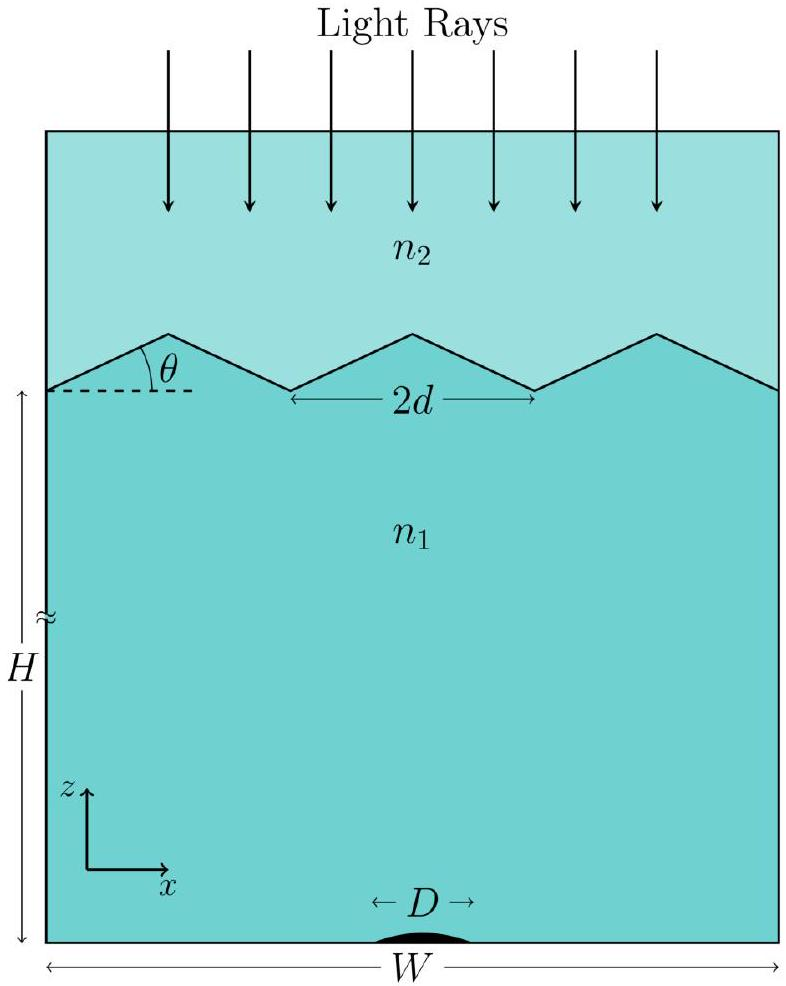
\includegraphics[max width=\textwidth, center]{2025_08_23_e94579452776a99c4850g-10}\\
    (T09.4) Consider an atmosphere modelled as above.\\
    (T09.4a) A section of the atmosphere with consecutive zigzag planes, with same parameters as stated above, is shown in the diagram below (not to scale).\\
    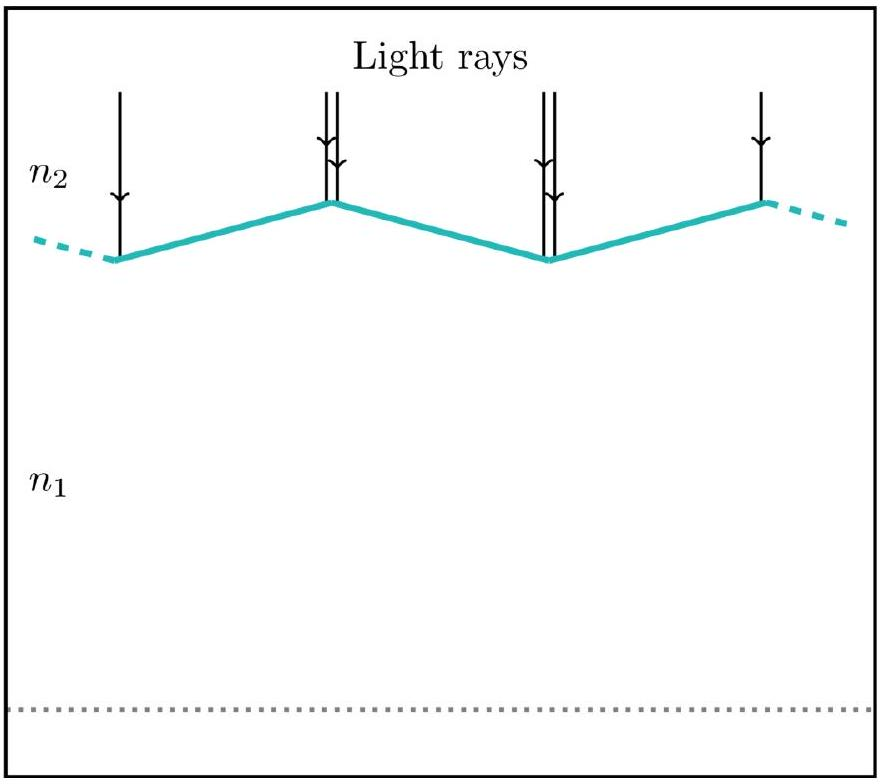
\includegraphics[max width=\textwidth, center]{2025_08_23_e94579452776a99c4850g-11}
    
    In this diagram, reproduced in the Summary Answersheet, draw the paths of the incident light rays up to the plane where the telescope objective is placed, shown by the gray dotted line.
    
    Mark the region(s), if any, by " X " in the diagram where no light rays will reach.\\
    (T09.4b) Calculate the width $W_{\mathrm{X}}$ of such region(s).\\
    (T09.4c) Find the largest diameter, $D_{\max }$, of the telescope objective with which it will be possible to obtain a single image of a star, by appropriately choosing the location of the telescope relative to the structure of the boundary.\\
    (T09.5) Consider the case when the zigzag shape of the boundary is allowed in both $x$ and $y$ directions\\
    (like a field of pyramids), and $D=100 \mathrm{~cm}$ (with $f=200 \mathrm{~cm}$ ).\\
    Draw the qualitative pattern of the resulting speckles in the box given in the Summary Answersheet.\\
    (T09.6) For a turbulent atmosphere again consider the same parallelly running zigzag shape of the boundary layer only along $x$-direction, but now the angle between two planes are changing at a uniform rate from $10^{\circ}$ to $-10^{\circ}$ in 1.0 s . Assume that this leads to a uniform rate of shift of the position of the image.
    
    Consider a telescope with $D=8 \mathrm{~cm}$ and $f=1 \mathrm{~m}$. Estimate the longest exposure time $t_{\text {max }}$ allowed for its CCD camera so that one gets only a single image, and any possible deviation in its position remains less than 1\% of the diffraction limited diameter of the image.\\

\end{document}